\documentclass{llncs}


\usepackage{listings}
\usepackage{textcomp}
\usepackage{xcolor}
\usepackage{enumitem}
\usepackage{amssymb}
\usepackage{empheq}
\usepackage{mathpartir}
% \usepackage{pxfonts}
\usepackage{fancybox}
\usepackage{algorithmic}
\usepackage{algorithm}
\usepackage[normalem]{ulem}
\usepackage{tikz}
\usepackage{reotex}
\usepackage{multicol}

\newcommand{\lang}{\emph{Mediator}}

\lstdefinelanguage{mediator}{
    keywords = {
        automaton,
        system,
        type,
        in, out,
        variables, transitions, statements, components, connections, 
        interface, func,
        sync,
        internals,
        begin, end,
        return,
        init, as,
        int, bool, char, enum, real
    },
    alsodigit = {-}
}

\lstset{
    basicstyle=\footnotesize\ttfamily,
    numbers=left,
    numberstyle=\scriptsize,
    columns=flexible,
    numbersep=10pt,
    tabsize=2,
    extendedchars=true,         %
    breaklines=true,
    keywordstyle=\bfseries,
    stringstyle=\color{white}\ttfamily, % Farbe der String
    xleftmargin=17pt,
    %xrightmargin=30pt,
    % frame=single,
    framexleftmargin=17pt,
    framexrightmargin=5pt,
    framexbottommargin=4pt,
    % backgroundcolor=\color{lightgray},
    showstringspaces=false,
    language=mediator,
    moredelim=**[is][\color{red}]{@}{@}
}

\newcommand\smalltitle[1]{
    \vspace{0.2cm}
    \noindent\emph{{#1}.}
}

\newcommand\T{\rule{0pt}{2.6ex}}       % Top strut
\newcommand\B{\rule[-1.2ex]{0pt}{0pt}} % Bottom strut

% terminal symbols
\newcommand{\tsym}[1]{\:\mbox{\texttt{#1}}\:}
% non-terminal symbols
\newcommand{\ntsym}[1]{\:\langle\mbox{\emph{#1}}\rangle\:}


\newcommand*\widefbox[1]{\fbox{\hspace{1em}#1\hspace{1em}}}

\newenvironment{bnf}{%
    \footnotesize
    % \vspace{-1em}
    \setkeys{EmphEqEnv}{align*}%
    \setkeys{EmphEqOpt}{box=\widefbox}%
    \EmphEqMainEnv%
}{
    \endEmphEqMainEnv
    % \vspace{-1em}
}
\long\def\CUT#1{\marginpar{CUT}} \long\def\CUT#1{\relax}

\title{Generating Arduino C Codes from \lang{}}
\author{Yi Li\and Meng Sun}
\institute{LMAM and Department of Informatics, School of Mathematical Sciences, \\ Peking University, Beijing, China \\
\email{liyi\_math@pku.edu.cn, sunmeng@math.pku.edu.cn}
}

\begin{document}
    \maketitle

    \begin{abstract}
        Manual encoding is exceedingly time consuming and error prone, and has become a huge obstacle between reliable software models and trustworthy computer programs. To deal with this problem, dozens of code generators are developed to automatically convert different models into executable codes. In this paper we present a new code generator for the component-based modeling language \lang{}. It aims to generate platform-dependent (Arduino in this case) programs that can be directly downloaded to the hardware without any manual adaption. We also present a case study where we use \lang{} to develop a wheeled-robot controller, generate the corresponding program through our code generator, which has been successfully executed on an Arduino-based robot platform.
        \keywords{Code Generation, Mediator, Arduino, Component-based Modeling}
    \end{abstract}
    
    \section{Introduction}

With IoT techniques sweeping around the world, software systems are becoming more complicated, distributed and safety-critical, and thus the development of such systems is becoming notoriously difficult. Small failures in daily-used software, such as smart house controllers, payment applications, etc., may lead to severe butterfly effect. Under such circumstances, various approaches have been proposed in the past decades to help software development, such as object-oriented programming \cite{SebestaConceptsOfPL}, aspect-oriented programming \cite{Kiczales1997}, component-based modeling and development \cite{SGM03}, and so on. Among these approaches, component-based modeling is extremely popular and helpful in the development of embedded systems \cite{Cmkovic2005} and service-oriented applications \cite{ACKM04}.

\lang{} \cite{LiFacsMediator2017} is a new component-based modeling language that provides an automata-based formal semantics and supports hierarchical modeling. With the help of a full-featured type system and powerful coordination mechanisms, this language can be used by both domain-specific experts and software engineers to guarantee the reliability of software system models.

However, such powerful modeling languages can only help with the correctness of high-level models. In practice, lots of software errors are caused by the inconsistency between implementations and models. And it turns out that manual implementations do not always precisely follow abstract models and designs, especially for systems with high complexity. To address this problem, automatic code generation has been proposed to avoid errors caused by human activities in the implementation process \cite{Budinsky1996}. In this paper, we present an algorithm that generates C code from \lang{} models, which can be directly compiled and executed on Arduino \cite{margolis2011arduino}, a popular open-source embedded platform.

%\smalltitle{Related Work} 
Importance of code generation has been uncovered for a long time. As a result, a large number of formal and industrial code generation tools have been built for different target platforms. For example, Event-B \cite{FisherNfmEventBJava2016} and SCADE \cite{BerryScp1992} are very popular formal tools that can generate executable codes from abstract models. The code generator in SCADE is especially famous for its reliability, but its scalablity is restricted by the Esterel language it accepts. As a synchronous language, Esterel only formalizes a single embedded control loop, which makes it hard to model concurrent and timed behavior. Furthermore, both Event-B and SCADE code generators only aim at x86 platform, i.e. they cannot generate code that directly works on embedded systems. 

On the other hand, Ptolemy\cite{PtolemyBook2014}, MATLAB Simulink Toolbox\cite{hahn2016essentialsimulink} and LabVIEW\cite{labview} are the most famous industrial modeling tools that support platform-dependent code generation. These tools have large number of libraries and plug-ins that almost cover all commonly-used embedded platforms and programming languages. Nevertheless, power of these tools also becomes limitation when we try to perform testing or verification techniques on their models. For example, Ptolemy uses standard JAVA as its semantics, and Simulink enables users to write components directly through MATLAB language. As far as we know, models directly written in such full-featured programming languages, with loop and dynamic memory allocation, are very hard to be verified.

The rest of this paper is structured as follows: Section \ref{sec:background} briefly introduces the \lang{} language and the Arduino platform. Then in Section \ref{sec:codegen} we illustrate how the \lang{}-Arduino code generator works. Section \ref{sec:experiment} presents the wheeled-robot controller as a case study. Finally, Section \ref{sec:conclusion} concludes the paper.
    \section{Background}
\label{sec:background}

\subsection{\lang{}}
\label{subsec:mediator}
\lang{} is a component-based modeling language proposed in \cite{LiFacsMediator2017}. As a hierarchical modeling language, \lang{} provides formalisms for both high-level \emph{system} layouts and low-level \emph{automata}-based behavior units. 

As implied by the name, the language tries to provide a mediator through different language elements. For example, \emph{system}s are designed for software engineers who may have no background about formal methods, which makes it easier to construct software models with reliable components and connectors. On the other hand, these reliable components and connectors are supposed to be built using \emph{automata} by researchers who know formal methods well.

Syntax tree of a typical \lang{} program is defined as follows.
\begin{bnf}
    \ntsym{program} ::=  (& \ntsym{typedef} | \ntsym{function} | \ntsym{automaton} | \ntsym{system})^*
\end{bnf}

\emph{Typedef}s are aliases for types. \emph{Function}s are definitions of custom (or \emph{native}, which will be interpreted later) functions. \emph{Automaton}s and \emph{system}s are the core modeling elements in \lang{}. They are also called \emph{entities} since they share the same declaration form. %More details of them are shown as follows.

\smalltitle{Type System} \lang{} provides various data types that are widely used in different formal modeling languages and programming languages. These data types are categorized as \emph{primitive types} and \emph{composite types}, which are presented in Table \ref{table:primitivetypes} and \ref{table:compositetypes}, respectively. \footnote{Some notations in Table \ref{table:primitivetypes} and \ref{table:compositetypes} are slightly different from the original language proposal in \cite{LiFacsMediator2017} since both the tool and language are still being frequently updated.}

\begin{table}
    \caption{Primitive Data Types}
    \label{table:primitivetypes}
    \centering
    \begin{tabular}{lcr}
        \hline
        Name & Declaration & Term Example \T\B \\
        \hline
        \T 
        Integer & \texttt{int} & \texttt{-1,0,1} \\
        Bounded Integer\hspace{0.5cm} & \texttt{int lowerBound .. upperBound}\hspace{0.5cm} & \texttt{-1,0,1} \\
        Double & \texttt{double} & \texttt{0.1, 1E-3} \\
        Boolean & \texttt{bool} & \texttt{true, false} \\
        Character & \texttt{char} & \texttt{'a', 'b'} \\
        \B Enumeration & \texttt{enum {item$_1$, ..., item$_n$}} & \texttt{enumname.item} \\
        \hline
    \end{tabular}
\end{table}
Table \ref{table:primitivetypes} shows the primitive types supported by \lang{}: \emph{integers and bounded integers, double values, boolean values, single characters} and \emph{finite enumerations}.
\begin{table}
    \caption{Composite Data Types (\texttt{T} denotes an arbitrary data type)}
    \label{table:compositetypes}
    \centering
    \begin{tabular}{lr}
        \hline
        Name & Declaration \T\B \\
        \hline
        \T Tuple  & \texttt{(T$_1$,...,T$_n$) }\\
        Union & \texttt{T$_1$|...|T$_n$ } \\
        Array & \texttt{T [length]}\\
        List & \texttt{T []} \\
        Map & \texttt{map [T$_{key}$] T$_{value}$} \\
        Struct\hspace{1cm} & \texttt{struct \{ field$_1$:T$_1$,..., field$_n$:T$_n$ \}} \\
        \B Initialized & \texttt{T$_{base}$ init term} \\
        \hline
    \end{tabular}
\end{table}

Composite types are used to construct complex data types from simpler ones. Such composite patterns in Table \ref{table:compositetypes} are interpreted as follows:
\begin{itemize}
    \item \emph{Tuple}. The \emph{tuple} operator `,' can be used to construct a finite tuple type with several base types.
    \item \emph{Union}. The \emph{union} operator `$|$' is designed to combine different types as a more complicated one. 
    \item \emph{Array} and \emph{List}. An \emph{array} $T[n]$ is a finite ordered collection containing exactly $n$ elements of type $T$. Moreover, a \emph{list} is an array of which the capacity is not specified, i.e. a list is a dynamic array.
    \item \emph{Map}. A \emph{map }[$T_{key}$] $T_{val}$ is a dictionary that maps a key of type $T_{key}$ to a value of type $T_{val}$.
    \item \emph{Struct}. A \emph{struct }\{$field_1:T_1,\cdots,field_n:T_n$\} contains a finite number of fields, each has  a unique identifier $field_i$ and a particular type $T_i$.
    \item \emph{Initialized}. An initialized type is used to specify the default value of a type $T_{base}$ with \texttt{term}.
\end{itemize}

\noindent\emph{Parameter Types}. In some situations we may hope to reuse an automaton or a system with the help of generalization. For example, an encrypted communication system supports different encryption algorithms encapsulated as parameter functions or components. Parameter types make it possible to take functions and entity interfaces as template parameters. \lang{} supports two parameter types: 
\begin{enumerate}
    \item \emph{Interface}, denoted by \texttt{interface (port$_1$:T$_1$,$\cdots,$port$_n$:T$_n$)}, defines a parameter that could be any \emph{automaton} or \emph{system} with exactly the same interface (i.e. number, types and directions of the ports perfectly match the declaration). Interfaces are only used in templates of \emph{system}s.
    \item \emph{Function Type}, denoted by \texttt{func (arg$_1$:T$_1$,$\cdots, $arg$_n$:T$_n$):T}, defines a function that has the argument types $\texttt{T}_1,\cdots,\texttt{T}_n$ and result type \texttt{T}. Functions are permitted to appear in templates of \emph{other functions}, \emph{automata} and \emph{system}s.
\end{enumerate}

Parameter types can only be used in template parameters. It is impossible to declare a function or an interface as a local variable.

\smalltitle{Functions} \lang{} supports two types of functions, \emph{common} functions and \emph{native} functions. The syntax of functions is shown as follows.

\begin{bnf}
    \ntsym{funcDecl} ::= & \tsym{native}^? \tsym{function} \ntsym{template}^? \ntsym{identifier} \ntsym{funcInterface} \tsym{\{} \\
    & (\tsym{variables} \tsym{\{} \ntsym{varDecl}^* \tsym{\}})^? \\
    & \tsym{statements} \tsym{\{} \ntsym{assignStmt}^* \ntsym{returnStmt} \tsym{\}} \\
    \ntsym{funcInterface} ::= & \tsym{(} (\ntsym{identifier} \tsym{:} \ntsym{type})^* \tsym{)} \tsym{:} \ntsym{type}\\
    \ntsym{assignStmt} ::= & \ntsym{term} (\tsym{,} \ntsym{term})^* \tsym{:=} \ntsym{term} (\tsym{,} \ntsym{term})^* \\
    \ntsym{iteStmt} ::= & \ntsym{if} \tsym{(} \ntsym{term} \tsym{)} \ntsym{stmt}^+ (\tsym{else} \ntsym{stmt}^+)^? \\
    \ntsym{returnStmt} ::= & \tsym{return} \ntsym{term} \\
    \ntsym{varDecl} ::= & \ntsym{identifier} \tsym{:} \ntsym{type} (\tsym{init} \ntsym{term})^? 
\end{bnf}


Common functions are composed of \emph{function interfaces} and \emph{function bodies}. Function interfaces describe the input variables and return type of functions. Function bodies, including local variables and statements, specify the behavior of the functions. All user-defined functions are common functions.

Native functions, on the other hand, have no function bodies but only function interfaces. Similar to the function declarations in other programming languages like C headers, native functions are part of the \lang{} plugins where the behavior of the functions cannot be described through \lang{} statements directly. For example, hardware-relevant operations, complex loops, etc. Such behavior can be captured by native codes in plugins. More discussions and examples of native functions will be presented in Section \ref{sec:codegen}.

\smalltitle{Entities} Both automata and systems are called \emph{entities} in \lang{}. All \lang{} entities %, no matter automata or systems, 
have their own templates and interfaces.  However, ways to formalize their behavior are complete different.

\smalltitle{Automata} Syntax tree of automata is shown as follows.
\begin{bnf}
    \ntsym{automaton} ::=& \tsym{automaton}\ntsym{template}^?\ntsym{identifier} \tsym{(} \ntsym{port}^* \tsym{)} \tsym{\{}\\
    & (\tsym{variables} \tsym{\{} \ntsym{varDecl}^* \tsym{\}})^? \\
    & \tsym{transitions} \tsym{\{} \ntsym{transition}^* \tsym{\}} \tsym{\}} \\
    \ntsym{port} ::=& \ntsym{identifier} \tsym{:} (\tsym{in}|\tsym{out}) \ntsym{type} \\
    \ntsym{transition} ::=& \ntsym{guardedStmt} | \tsym{group} \tsym{\{} \ntsym{guardedStmt}^* \tsym{\}}\\
    \ntsym{guardedStmt} ::=& \ntsym{term} \tsym{->} (\ntsym{stmt} | \tsym{\{} \ntsym{stmt}^* \tsym{\}}) \\
    \ntsym{stmt} ::=& \ntsym{assignStmt} | \ntsym{iteStmt} | \tsym{sync} \ntsym{identifier}^+\\
\end{bnf}

As the basic behavior unit in \lang{}, \emph{automaton} consists of four parts: \emph{templates}, \emph{interfaces}, \emph{local variables} and \emph{transitions}, which are interpreted respectively as follows.
\begin{enumerate}
    \item \emph{Templates}. Templates of an automaton include a set of parameter declarations. A parameter can be either a type (common type or parameter type) or a value. Concrete values or types are supposed to be provided when the automaton is instantiated (i.e. declared in systems).
    \item \emph{Interfaces}. Interfaces consist of directed ports and describe how automata interact with their contexts. Ports can be regarded as structures with three fields: \texttt{value}, \texttt{reqRead} and \texttt{reqWrite}, which correspondingly denote the values of parts, status of reading requests and status of writing requests.
    \item \emph{Local Variables}. Each automaton contains a set of local variables. Types of these variables are supposed to be \emph{initialized}. We use the evaluations of local variables to represent states of an automaton.
    \item \emph{Transitions.} Behavior of an automaton is depicted by guarded transitions. Each transition consists of a boolean term \emph{guard} and a sequence of statements. Transitions are ordered by their priority. For example, if multiple transitions are activated at the same time, the one that has highest priority will be fired. On the other hand, non-deterministic firing is also supported by encapsulating part of the transitions through \texttt{group}. 
\end{enumerate}

Currently, \lang{} supports three types of statements:
\begin{enumerate}
\item \emph{Assignment} statements, each including an expression and an optional assignment target, evaluate the expression and assign the result to its target if possible. 
\item \emph{Ite} (if-then-else) statements act as conditional choice statements in other languages. 
\item \emph{Synchronizing} statements, labelled with \texttt{sync}, are the flags requiring synchronized communication with other entities. 
\end{enumerate}
According to the existence of synchronizing statement (i.e. external communication through ports), transitions are classified as either \emph{internal} transitions or \emph{external} ones.

Compared with automata models being widely-used in other formal tools (e.g. UPPAAL\cite{AmnellMovepUppaal2001}, Simulink/Stateflow\cite{hahn2016essentialsimulink}), an automata in \lang{} has no explicitly declared locations. Instead, it uses the evaluation of local variables to represent its states. An example of \lang{} automaton can be found in Example \ref{exp:automaton}, Section \ref{sec:experiment}, where automata are used to model drivers of motors.

\begin{bnf}
    \ntsym{system} ::= & \tsym{system} \ntsym{template}^?\ntsym{identifier} \tsym{(} \ntsym{port}^* \tsym{)} \tsym{\{}\\
    & (\tsym{internals} \ntsym{identifier}^+)^? \\
    & (\tsym{components} \tsym{\{} \ntsym{componentDecl}^* \tsym{\}})^? \\
    & \tsym{connections} \tsym{\{} \ntsym{connectionDecl}^* \tsym{\}} \tsym{\}}\\
    \ntsym{componentDecl} ::= & \ntsym{identifier}^+ \tsym{:} \ntsym{systemType} \\
    \ntsym{connectionDecl} ::= & \ntsym{systemType} \ntsym{params} \tsym{(} \ntsym{portName}^+ \tsym{)}
\end{bnf}

\smalltitle{Systems} As the textual representation of hierarchical entities to organize sub-entities (automata and simpler systems), \emph{systems} with the above syntax tree are composed of:
\begin{enumerate}
    \item \emph{Components}. Entities can be placed and instantiated in systems as components. Each component is considered as a unique instance and executed in parallel with other components and connections. Ports of a component can be referenced by \texttt{identifier.portName} once the component is declared.
    \item \emph{Connections}. Connections are used to connect \emph{a) the ports of the system itself, b) the ports of its components, and c) the internal nodes}. Inspired by the Reo project\cite{ArbabMscsReo2004,Arbab2007,BaierScp2006}, complex connection behavior can also be determined by other entities.
    \item \emph{Internals}. Sometimes we need to combine multiple connections to perform more complex coordination behavior. Internal nodes, declared in \texttt{internals} segments, are untyped identifiers which are capable to weld two ports with consistent data-flow direction.
\end{enumerate}

Systems also have \emph{templates} and \emph{interfaces} which have exactly the same forms as in automata. An example of a \lang{} system is presented later in %Example \ref{exp:system}, 
Section \ref{sec:experiment}.

\subsection{Arduino}
\label{subsec:arduino}

Arduino\cite{margolis2011arduino} is an open-source electronics project that aims to build easy-to-use hardware and software. Arduino boards support various models of single-board micro-controllers, properly encapsulate them and expose a set of simple APIs to users. Here we give a brief introduction on program structure of Arduino C and hardware resources on a typical Arduino motherboard.

\smalltitle{Program Structure}
The Arduino community has developed a simple IDE that uses a dialect of C as its programming language. A typical Arduino C program describes its behavior through a \texttt{setup} function and a \texttt{loop} function. 
%An example of Arduion C program is in Example \ref{exp:arduinoprog}.
\begin{itemize}
    \item \texttt{setup()}: This function is called once when a sketch starts after power-up or reset. It is used to initialize variables, input and output pin modes, and other libraries needed in the sketch.
    \item \texttt{loop()}: After \texttt{setup} has been called, function \texttt{loop} is executed repeatedly in the main program. It controls the board until the board is powered off or is reset.
\end{itemize}

\smalltitle{Hardware Resources} Pins are the most import hardware resources of Arduino boards. Through them the motherboard communicates with its accessories, e.g. sensors, motors and other devices. Numbers and types of pins vary a lot between different Arduino motherboards. Here we take Arduino Uno, one of the most popular Arduino motherboards, as an example to introduce types of pins. This motherboard is also used for the case study in Section \ref{sec:experiment}.

\begin{enumerate}
    \item \emph{Analog Pins}: 6 analog pins named \texttt{A0 .. A5} are provided on Arduino Uno to perform analog signal transmission. Resolution of analog pins is 10 bits, in other words, value of an analog pin varies from $0$ to $1023$. Reading and writing operations on analogs pins are performed through builtin functions \texttt{analogRead(pin)} and \texttt{analogWrite(pin,value)}.
    \item \emph{Digital Pins}: Digital pins have only two possible values $0$ and $1$, or \texttt{LOW} and \texttt{HIGH}. Builtin functions \texttt{digialRead} and \texttt{digitalWrite} are used to read values from and write values to digital pins. Moreover, part of the digital pins provide Pulse-Width Modulation (PWM, \cite{linkpwm}) feature to transfer analog value through binary encoding. In this case we are supposed to use \texttt{analogRead} and \texttt{analogWrite} instead.
\end{enumerate}

An Arduino pin can be in either \emph{INPUT} mode or \emph{OUTPUT} mode. Modes of pins, no matter whether they are analog or digital, are configured through the builtin function \texttt{pinMode(pin, mode)}.

\CUT{
\begin{example}[A Minimized Arduino C Program]
    \label{exp:arduinoprog}
    The following program from \cite{margolis2011arduino} flashes the onboard LED light periodically through changing the electronic level of pin 13.
\begin{lstlisting}
#define LED_PIN 13                  // Pin number attached to LED.

void setup() {
    pinMode(LED_PIN, OUTPUT);       // Set pin 13 as a digital output.
}

void loop() {
    digitalWrite(LED_PIN, HIGH);    // Turn on the LED.
    delay(1000);                    // Wait 1 second (1000 milliseconds).
    digitalWrite(LED_PIN, LOW);     // Turn off the LED.
    delay(1000);                    // Wait 1 second.
}
\end{lstlisting}
\end{example}
}
    \section{Code Generation}
\label{sec:codegen}

In this section we introduce the Arduino code generator for \lang{}. The code generator mainly consists of a native function library and a set of generators for different \lang{} language elements, e.g. types, functions and entities.

The Arduino code generator is implemented as a plugin of the \lang{} project \cite{medgit}, which is written in Java and based on Maven framework. Executable Jar packages and help documents can be found in this repository.

\subsection{Native Functions}

Native functions are the bridges between software controllers and hardware resources in the \lang{} framework. It tells \lang{} which and how the hardware resources can be operated. Similar to C/C++ header files, these native functions are declared in a \lang{} source file as a library. But their corresponding hardware behavior is defined by the code generator plugin.

The Arduino code generator supports the following native functions:
\begin{lstlisting}
native function digitalRead (pin: int) : int 0..1;
native function digitalWrite (pin: int, val:int 0..1);
native function analogWrite (pin: int) : int 0..1023;
native function analogWrite (pin: int, val:int 0..1023);
native function delay (milliseconds: int);
\end{lstlisting}
\begin{itemize}
    \item \emph{DigitalRead} reads binary signals from a digital pin.
    \item \emph{DigitalWrite} writes binary signals to either a digital or an analog pin. When it is performed on an analog pin, it configures the analog electronic level to either $1023$ (\texttt{HIGH}) or $0$ (\texttt{LOW}).
    \item \emph{AnalogRead} reads analog signals from an analog pin.
    \item \emph{AnalogWrite} writes analog signals to either an analog pin or a digital pin that supports PWM encoding.
    \item \emph{Delay} forces the Arduino processor to suspend for a certain time delay.
\end{itemize}

\subsection{Type Generator}

Arduino C naturally supports most of the primitive types in Table \ref{table:primitivetypes} and part of the composite types in Table \ref{table:compositetypes}: unbounded integers \texttt{int}, float point numbers \texttt{double}, characters \texttt{char}, boolean values \texttt{bool} (as zero and non-zero integers), enumeration \texttt{enum}, union \texttt{union}, structure \texttt{struct} and finite arrays.

For the other types that are not directly supported by Arduino C, we use an attached runtime library to simulate their behavior. Such types include:

\begin{itemize}
    \item \emph{Bounded Integer}. In \lang{}, bounded integers are mainly used to avoid overflow and unexpected values. For example, an Arduino analog signal varies between $0$ and $1023$, writing any other integers to an analog pin may lead to unknown behavior. Bounded integers are not supported by C. Moreover, according to its widely use we may suffer from performance degradation if we use complex structures to represent them. So we choose to generate assertions every time when a variable of bounded integer type is assigned. For example,
    \begin{lstlisting}[language=C]
int a = 0;  // type of a is int 0 .. 1 init 0
void loop() {
    // ...
    a = 1 - a;
    assert (a >= 0 && a <= 1);
    // ...
}
    \end{lstlisting}
    \item \emph{List}. C supports unbounded lists by pointers. However, C does not care about the capacity and consumption of them, which frequently lead to memory overflow and invalid dereference. In the \lang{} runtime library, we encapsulate a void pointer to represent an unbounded list, and two integer fields to denote its capacity and the number of items existing in this list.
    \begin{lstlisting}
struct __MR_List {
    void * list;
    int capacity;
    int num_items;
    int item_size;
};
typedef struct __MR_List MR_List;

void init_empty_list (MR_List list, int item_size);
void list_add (MR_List list, void * item);
void * list_get (MR_List list, int index);
void list_del (MR_List list, int index);
    \end{lstlisting}
    The definition of unbounded list, as shown here, is type-independent. In other words, when storing items to or obtaining items from an unbounded list, type casting is unavoidable. In this case the \lang{} syntax checker is responsible to guarantee the type consistency.
    \item \emph{Map}. Similar to the \emph{list}, \lang{} \emph{map} in Arduino C is also type-independent. A map uses two unbounded lists to store keys and values, respectively.
    \begin{lstlisting}
struct __MR_Map {
    MR_List keys;
    MR_List values;
};
typedef struct __MR_Map MR_Map;

void init_empty_map (MR_Map map, int key_size, int value_size);
void map_put (MR_Map map, void * key, void * value);
void * map_get (MR_Map map, void * key);
void map_del (MR_Map map, void * key);      
    \end{lstlisting}
    \item \emph{Initialized}. In an Arduino program, default value of a type is only used in the \texttt{setup} function to initialize the corresponding variable. As a result, we do not have to use initialized type in Arduino C explicitly. For example, \texttt{int init 0} will be simply replaced by \texttt{int} when the Arduino C code is generated.
\end{itemize}

\subsection{Function Generator}

As mentioned before, there are two types of functions to be considered here: common functions and native functions.

\smalltitle{Common Functions} When designing \lang{}, we deliberately restrict the expressiveness of common functions (transitions as well) so that they are easier to be verified formally. As a result, common functions in \lang{} are very easy to be encoded in C.

\smalltitle{Native Functions} When a native function is called in a transition, the code generator needs to replace the function with corresponding native API in Arduino C. According to Section \ref{subsec:arduino}, all native functions supported in this plugin can be mapped to an Arduino API with the same name.

\subsection{Entity Generator}

All Arduino motherboards are equipped with only one processor and there is no time-sharing operating system support. They do not support parallel execution. Consequently, typical \lang{} systems including a set of parallel components and connections can not be directly encoded in Arduino C.

Fortunately, a scheduling algorithm that flats a hierarchical system into a single automaton has been introduced in \cite{LiFacsMediator2017}. The algorithm guarantees that its resulting automaton is always canonical, i.e., the automaton 
contains exactly one transition group, in which all transitions are also canonical. With help of this algorithm, all we 
need to do is to encode a single \lang{} automata in Arduino C. 

The following steps illustrate the sketch of the encoding process.

\begin{enumerate}
    \item \emph{Template and Interface}. When generating Arduino codes, we always assume that the source automaton has NO template parameters and NO ports. Ports are special elements in \lang{} that are used to react with a \lang{} context. Behavior of ports are undeclared in the Arduino C context.
    \item \emph{Local variables} are declared as global variables in Arduino C. According to \cite{LiFacsMediator2017}, types of all local variables should be initialized, i.e., they are declared with default values. And these default values will be assigned to the global variables in the \texttt{setup} function.
    \item \emph{Statements}. Transitions are composed of sequences of statements. After being scheduled and canonicalized, an automaton contains only \emph{assignment statements} and \emph{ite statements} (which are inherently supported in C). Since we assume that no port exists in the automaton's interface, \emph{synchronizing statements} can be simply omitted. 
    \item \emph{Transitions}. Transitions are \emph{activated} if their guards are satisfied by the current evaluation of the local variables. Since in a canonical automaton all transitions are encapsulated by a \texttt{group}, the transition selection process is fully non-deterministic, i.e. the transition to fire is randomly selected from all \emph{activated} transitions. In our approach, we use the following three steps to perform transition selection and firing:
    \begin{itemize}
        \item Step 1. \emph{Activation checking}. At the beginning of each \texttt{loop}, we use a set of \texttt{if} statements to check which transitions are activated under the current evaluation of local variables. We use an array \texttt{cmd\_activated} to store indexes of all transitions being activated.
        \item Step 2. \emph{Random selection}. With the help of the \texttt{random} function in Arduino, it is easy to pick up a random index number from \texttt{cmd\_activated}.
        \item Step 3. \emph{Transition firing}. Another set of \texttt{if} blocks are used to encode the statements in transitions. Conditions of these blocks are used to check whether index of this transition is equal to the selected index.
    \end{itemize}
\end{enumerate}

\begin{example}
    Consider a \lang{} automaton \texttt{test} with one local variable $x$ (initialized by $0$) and two transitions: increasing $x$ by $1$ if $x$ is less than zero, or decreasing $x$ by $1$ otherwise. The generated Arduino C code is as follows.
    \begin{lstlisting}
int test_x;
int cmd; // stores the index of selected transition
int cmd_activated[1]; // the capacity depends on number of transitions that belongs to the automaton

void setup() { test_x = 0; }

void loop() {
    // STEP 1 collect activated transitions
    cmd_activated_counter = 0; // the stack pointer of cmd_activated
    if (test_x < 0) {
        cmd_activated[cmd_activated_counter] = 0;
        cmd_activated_counter ++;
    }
    if (test_x >= 0) {
        cmd_activated[cmd_activated_counter] = 1;
        cmd_activated_counter ++;
    }

    // STEP 2 pick up a transition randomly
    cmd = cmd_activated[random(cmd_activated_counter)];

    // STEP 3 fire the selected transition
    if (cmd == 0) test_x = test_x + 1;
    if (cmd == 1) test_x = test_x - 1;
}
    \end{lstlisting}
\end{example}
The code generating process is summarized in Algorithm \ref{alg:generate}.

\begin{algorithm}[ht]
    \caption{Generate Codes for a Specified Entity $E$ in a Program $P$}
    \label{alg:generate}
    \algsetup{linenosize=\small}
    \small
    \begin{algorithmic}[1]
        \REQUIRE A program $P=\langle Typedefs, Functions, Automata, Systems\rangle$, an entity $E$
        \ENSURE Arduino C codes
        \STATE $global, setup, loop\leftarrow$ ``\; ''
        \IF {$E\in Automata$}
            \STATE $A \leftarrow \texttt{Canonicalize}(E)$
        \ELSE
            \STATE $A \leftarrow \texttt{Schedule}(E)$
        \ENDIF
        \IF {$A.Ports\neq\varnothing$}
            \RETURN{NULL}
        \ENDIF
        \FOR {$var\in\{$local variables of $A\}$}
            \STATE add variable declaration of $var$ to $global$ with the generated type
            \STATE add variable initialization of $var$ to $setup$
        \ENDFOR
        
        \FOR{$t=guard\rightarrow statements\in \{$transitions of $A\}$}
            \STATE add activation checking of $guard$ to $loop$
        \ENDFOR

        \STATE add \emph{random index selection} to $loop$

        \FOR{$t=guard\rightarrow statements\in \{$transitions of $A\}$}
            \STATE add the generated $statements$ to $loop$
            \IF {pin $pin$ is involved in $statements$}
                \STATE add \texttt{pinMode} to $setup$ to configure $pin$ correctly
            \ENDIF
        \ENDFOR
        \STATE $setup \leftarrow$ ``\texttt{void setup()\{}'' + $setup$ + ``\texttt{\}}''
        \STATE $loop \leftarrow$ ``\texttt{void loop() \{}'' + $loop$ + ``\texttt{\}}''
        \RETURN $global+setup+loop$
    \end{algorithmic}
\end{algorithm}
    \section{Experiment}
\label{sec:experiment}

In this section, we show how to model a wheeled-robot controller in \lang{} and generate Arduino C code through our code generator. The generated platform-dependent code has been directly compiled and flashed to the motherboard, without any manual modification.

The hardware platform being used is based on an Arduino Uno motherboard, which consists of 4 motors (divided into two group \em{left} and \em{right}) and an ultrasonic distance sensor, as shown in Fig.~\ref{img:circuits}.

\begin{figure}[!ht]
    \centering
    % \begin{minipage}[t]{0.4\linewidth}
        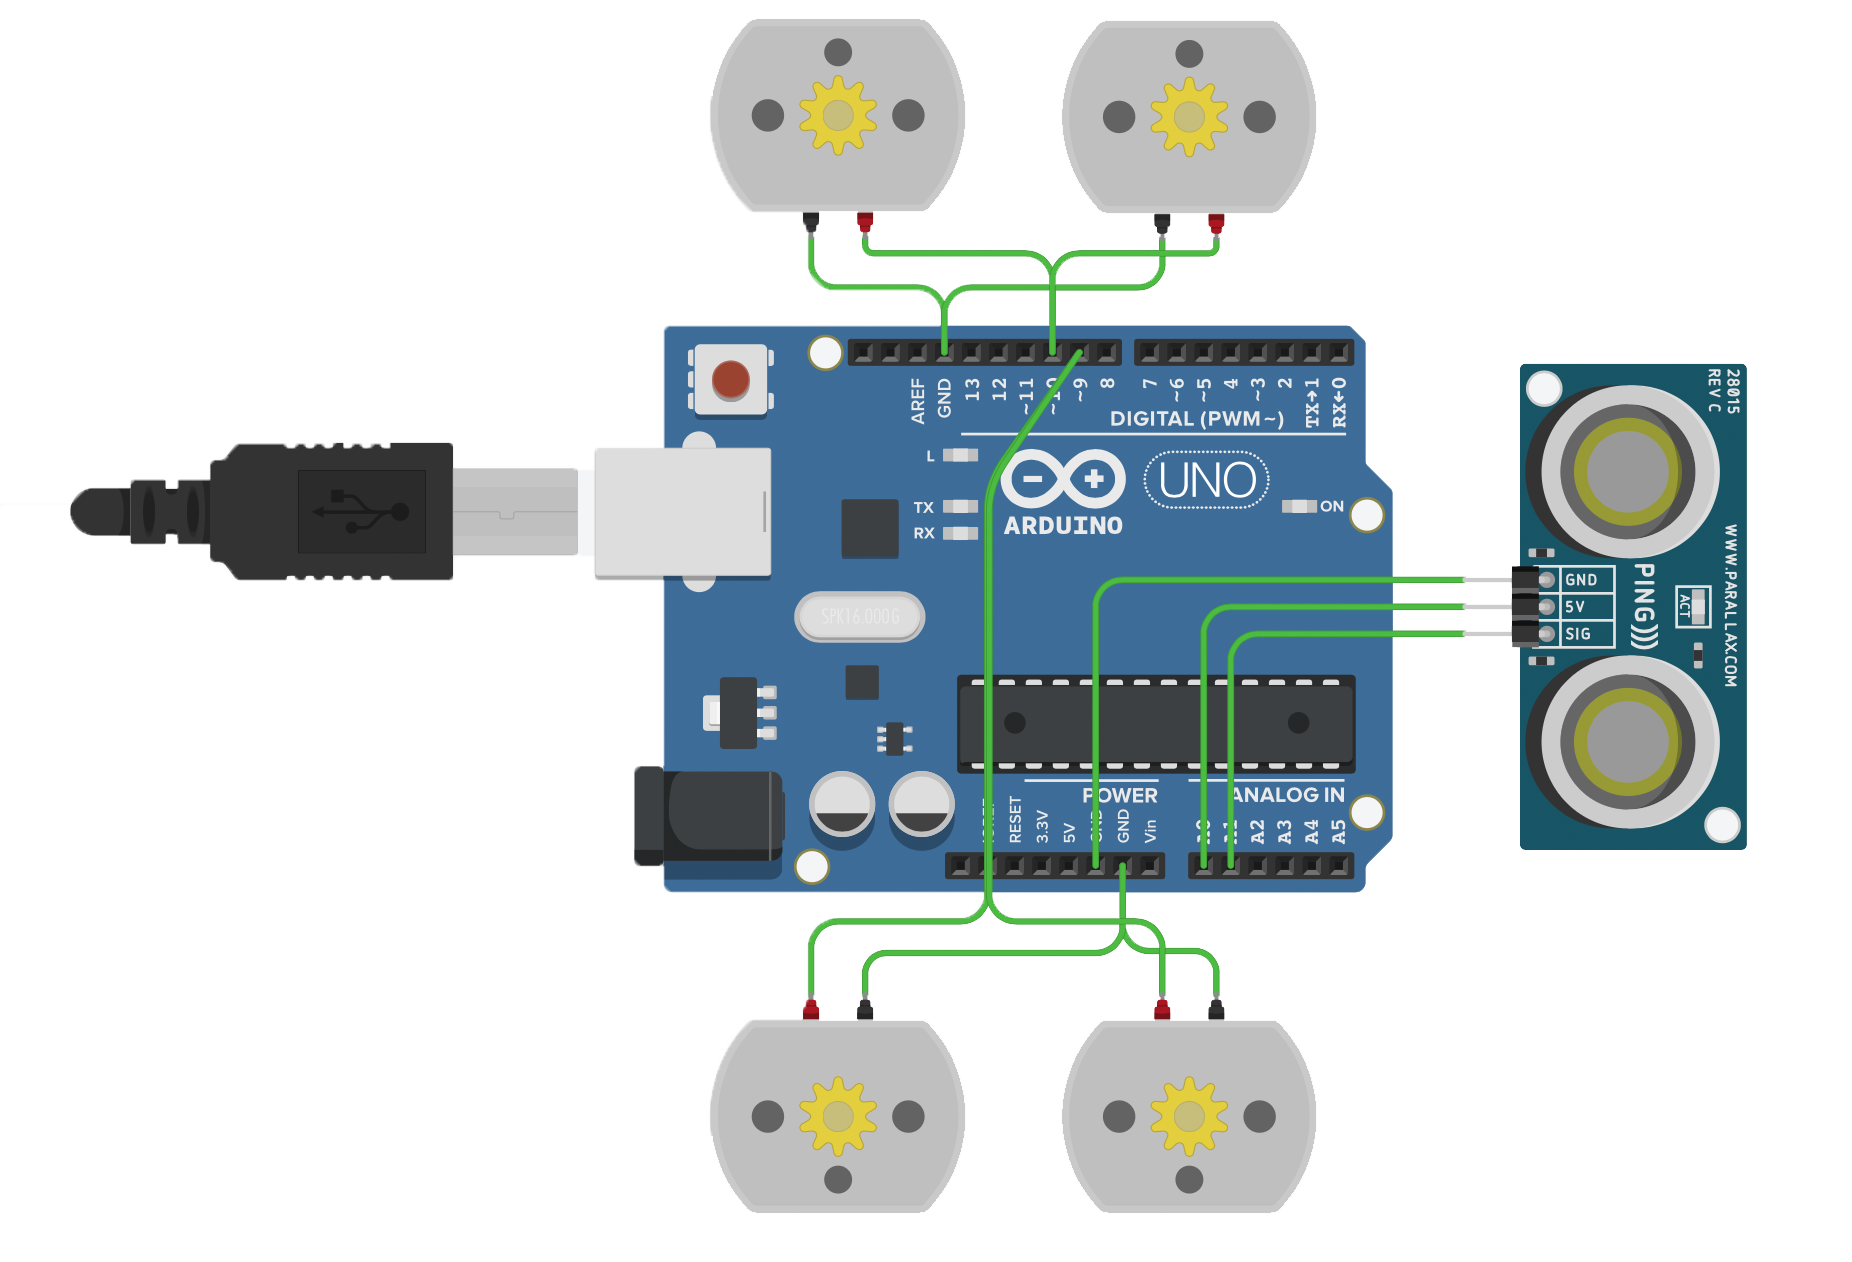
\includegraphics[width=.5\textwidth]{images/circuits.png}
    % \end{minipage}
    % \begin{minipage}[t]{0.4\linewidth}
        % 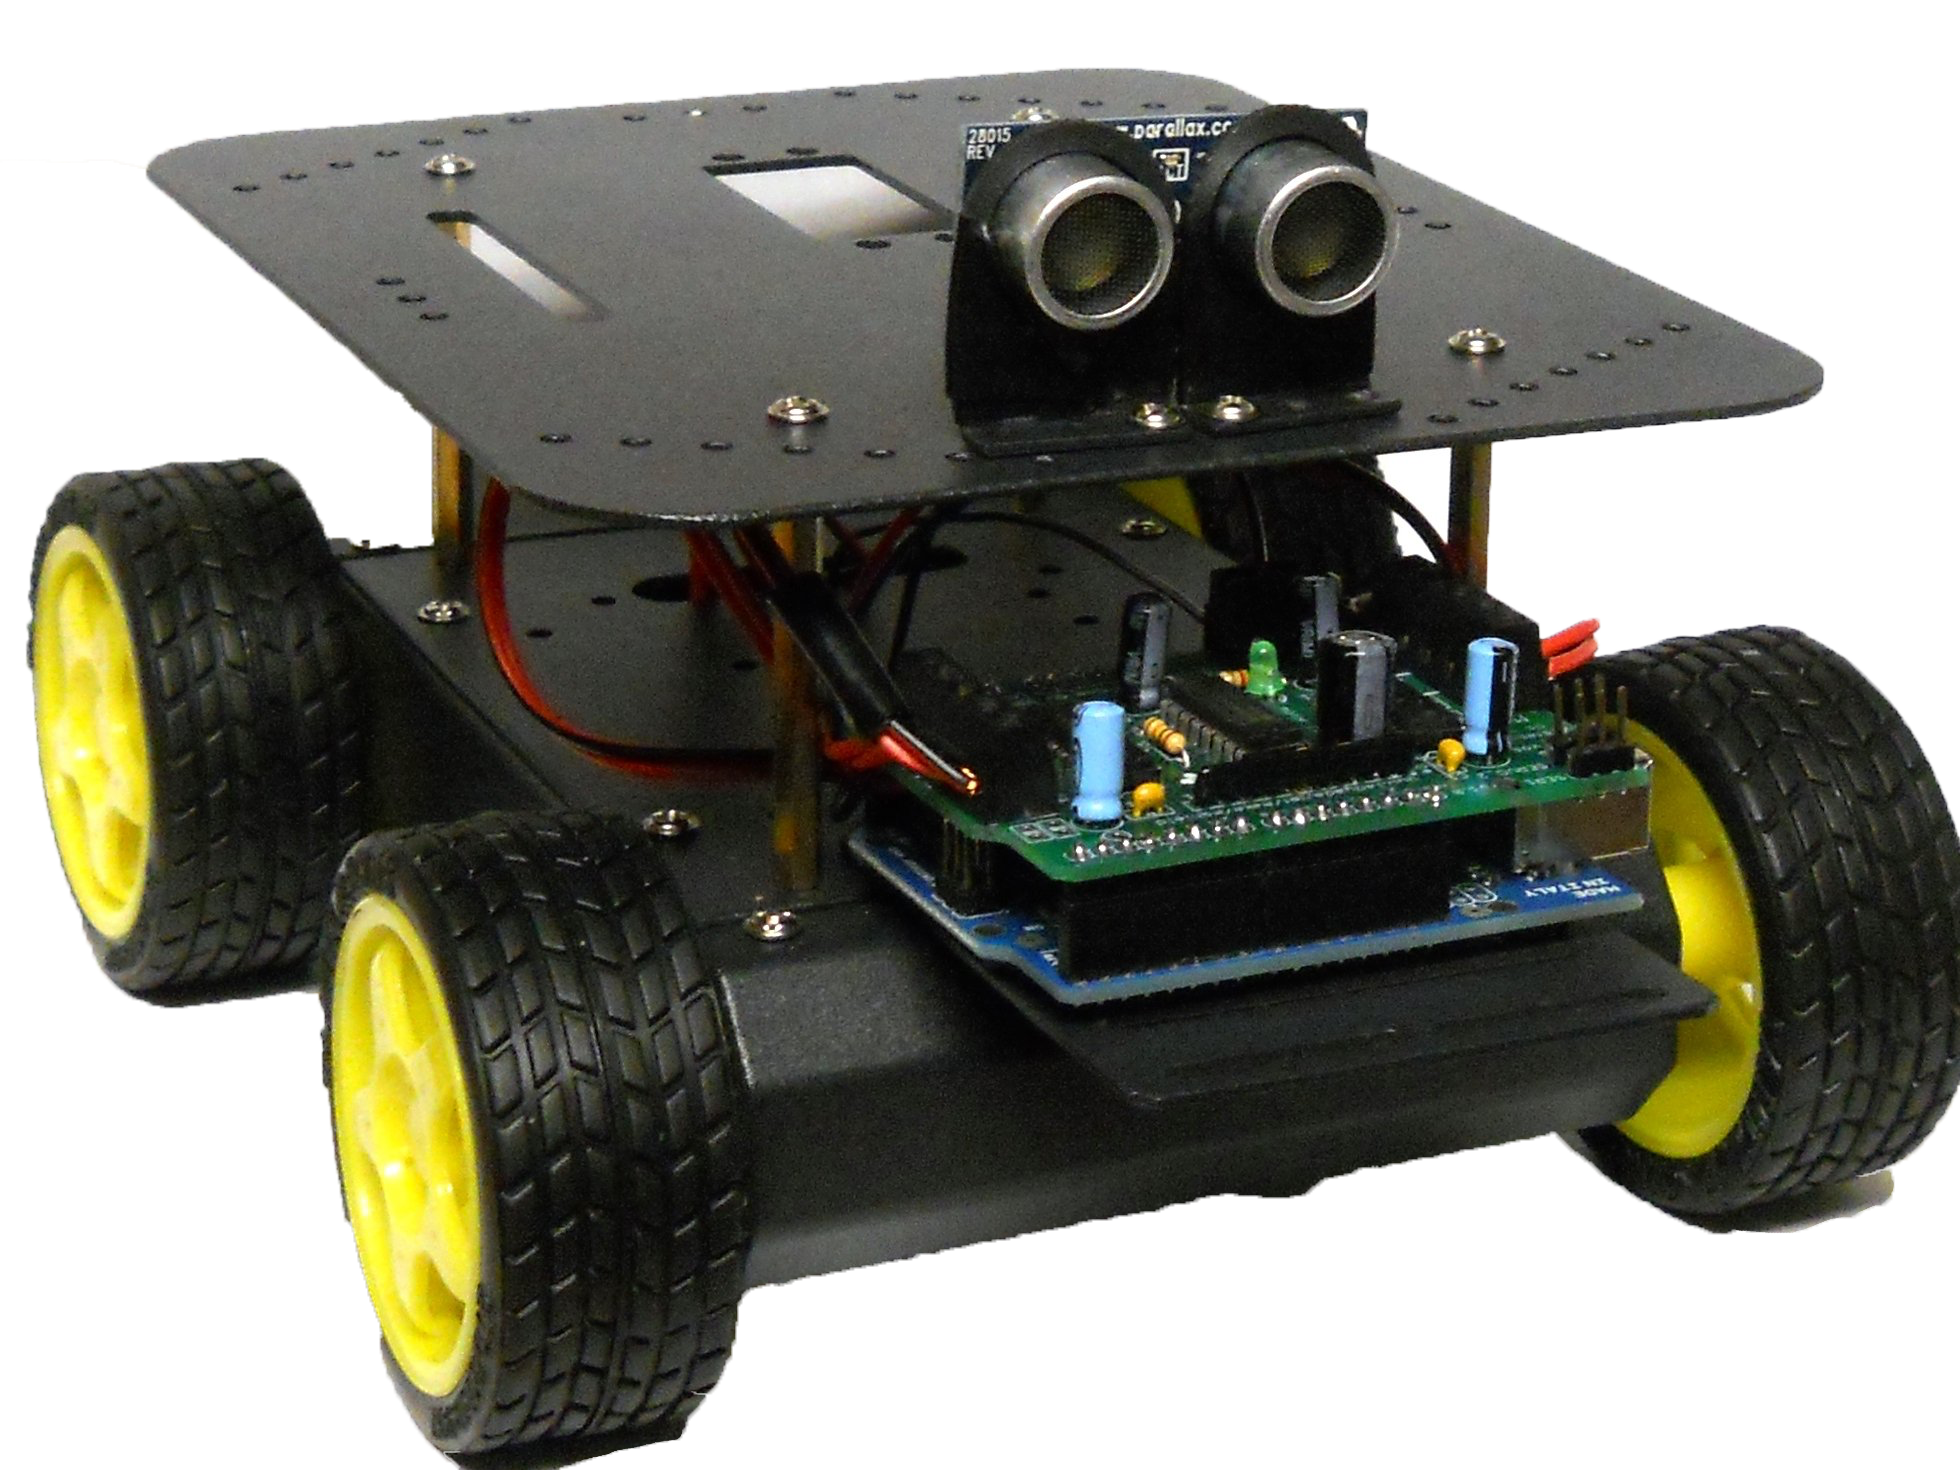
\includegraphics[width=.9\textwidth]{images/robot.png}
    % \end{minipage}
    \caption{Hardware Architecture of the Experiment Platform}
    \label{img:circuits}
\end{figure}

%\subsection{Formal Model in \lang{}}

The \lang{} model of the wheeled-robot controller as shown in Figure \ref{img:controller} contains the following parts:

\begin{itemize}
    \item \emph{UltraSonic}. This sensor detects the distance from nearest obstacles and sends the distance information to the controller.
    \item \emph{Controller}. The core algorithm of this robot is encapsulated in the controller. It reads distance information from the ultrasonic sensor, and gives an abstract command (e.g. forward, backward, turn, stop) to the \emph{speeder} according to the distance information.
    \item \emph{Speeder}. This automaton updates the speed of two motor groups according to the abstract command it receives from the \emph{controller}.
    \item \emph{Motors}. 4 motors, divided into two groups, are equipped in this small robot. Each motor has two control pins, one for direction and the other for speed. The \lang{} automaton shown in Example \ref{exp:automaton} is the driver for motors. It receives a single control signal \emph{speed} and updates the electronic level of control pins correspondingly.
\end{itemize}

\begin{figure}[ht]
    \centering
    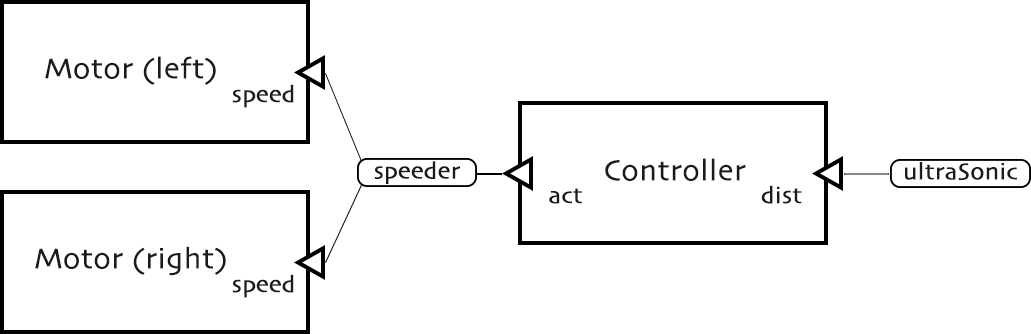
\includegraphics[width=.8\textwidth]{images/architecture.png}
    \caption{Mediator Model of the Robot Controller}
    \label{img:controller}
\end{figure}

%\begin{example}[Robot Controller] 
The controller shown in Figure \ref{img:controller} is captured by the following \lang{} code, where the motors and the controller are defined as components, and the speeder and ultrasonic distance sensor are defined as connections.
    \label{exp:system}
\begin{lstlisting}
system robot () {
    components {
        left_motor : motor<8, 9>;
        right_motor : motor<11, 10>;
        c  : controller;
    }
    connections {
        speeder(c.act, left_motor.speed, right_motor.speed);
        ultraSonicDist<6,7>(c.dist);
    }
}
\end{lstlisting}
%\end{example}

Four \lang{} automata are specified in this controller model: \emph{motor}, \emph{controller}, \emph{speeder} and \emph{ultraSonicDist}. Here we only show the definition of \emph{motor}, further details can be found at \cite{medgit}.

%\begin{example}[Motor Driver]
%    \label{exp:automaton}
    A typical driver of motors with two control signals is defined as an automaton in \lang{}. The simple automaton contains no local variable, one internal transition and one external transition. The internal transition updates the status of port \texttt{speed}, which is supposed to be ready to accept control commands at anytime. And the external transition receives target speed from the \texttt{speed} port and gives orders to the hardware correspondingly. The two template parameters describe where Arduino pins the motor is connected.
    \begin{lstlisting}
automaton <pinDirection,pinSpeed:int> motor (speed:in signedPWM) {
    variables {}
    transitions {
        !speed.reqRead -> speed.reqRead = true; // internal
        speed.reqRead && speed.reqWrite -> {
            sync speed; // external communication flag
            if (speed.value > 0) {
                digitalWrite(pinDirection, 1);
                analogWrite(pinSpeed, speed.value);
            } else {
                digitalWrite(pinDirection, 0);
                analogWrite(pinSpeed, -speed.value);
            }
        }
    }
}
    \end{lstlisting}
%\end{example}

%\subsection{Generated C Codes}

Due to the length limitation, the generated program is omitted here and can be found at \url{https://github.com/mediator-team/codegen-proposal/experiment}.
    \section{Conclusion and Future Work}
\label{sec:conclusion}

In this paper, we developed a fully-automatic code generator that converts \lang{} models to executable Arduino C programs. Compared with plain Arduino C code, component-based \lang{} models are more intuitive, easier to understand and construct. With the help of this code generator, engineers are able to build and review their models in \lang{}, and generate Arduino C code automatically to avoid errors caused by manual encoding.

%\smalltitle{Future Work} Our future works are listed as follows.
%\begin{enumerate}
In the future we plan to use program verification tools to guarantee the reliability of generate codes.  Due to the complexity, it is hard to formally prove the correctness of the code generator itself. So we plan to generate assertions automatically and insert them into the target code for formal verification. Hopefully they can be verified through program verification tools, e.g. CBMC\cite{Clarke2004}.
Providing support for more hardware platforms and languages, e.g. Verilog/VHDL, System C, etc., are in our scope as well.
%\end{enumerate}

\section*{Acknowledgement}
The work was partially supported by the National Natural Science Foundation of China under grant no. 61772038, 61532019, 61202069 and 61272160.

    \bibliographystyle{splncs03}
    \bibliography{library,local}    

\end{document}